\documentclass[12pt,modern]{article}
\usepackage{fancyhdr}
\usepackage{graphicx}
\usepackage[margin=1in]{geometry}

\pagestyle{fancy}
\fancyhf{}
\lhead{AU Mic Research Overview}
\rhead{Cail Daley}

\begin{document}

\begin{figure}
  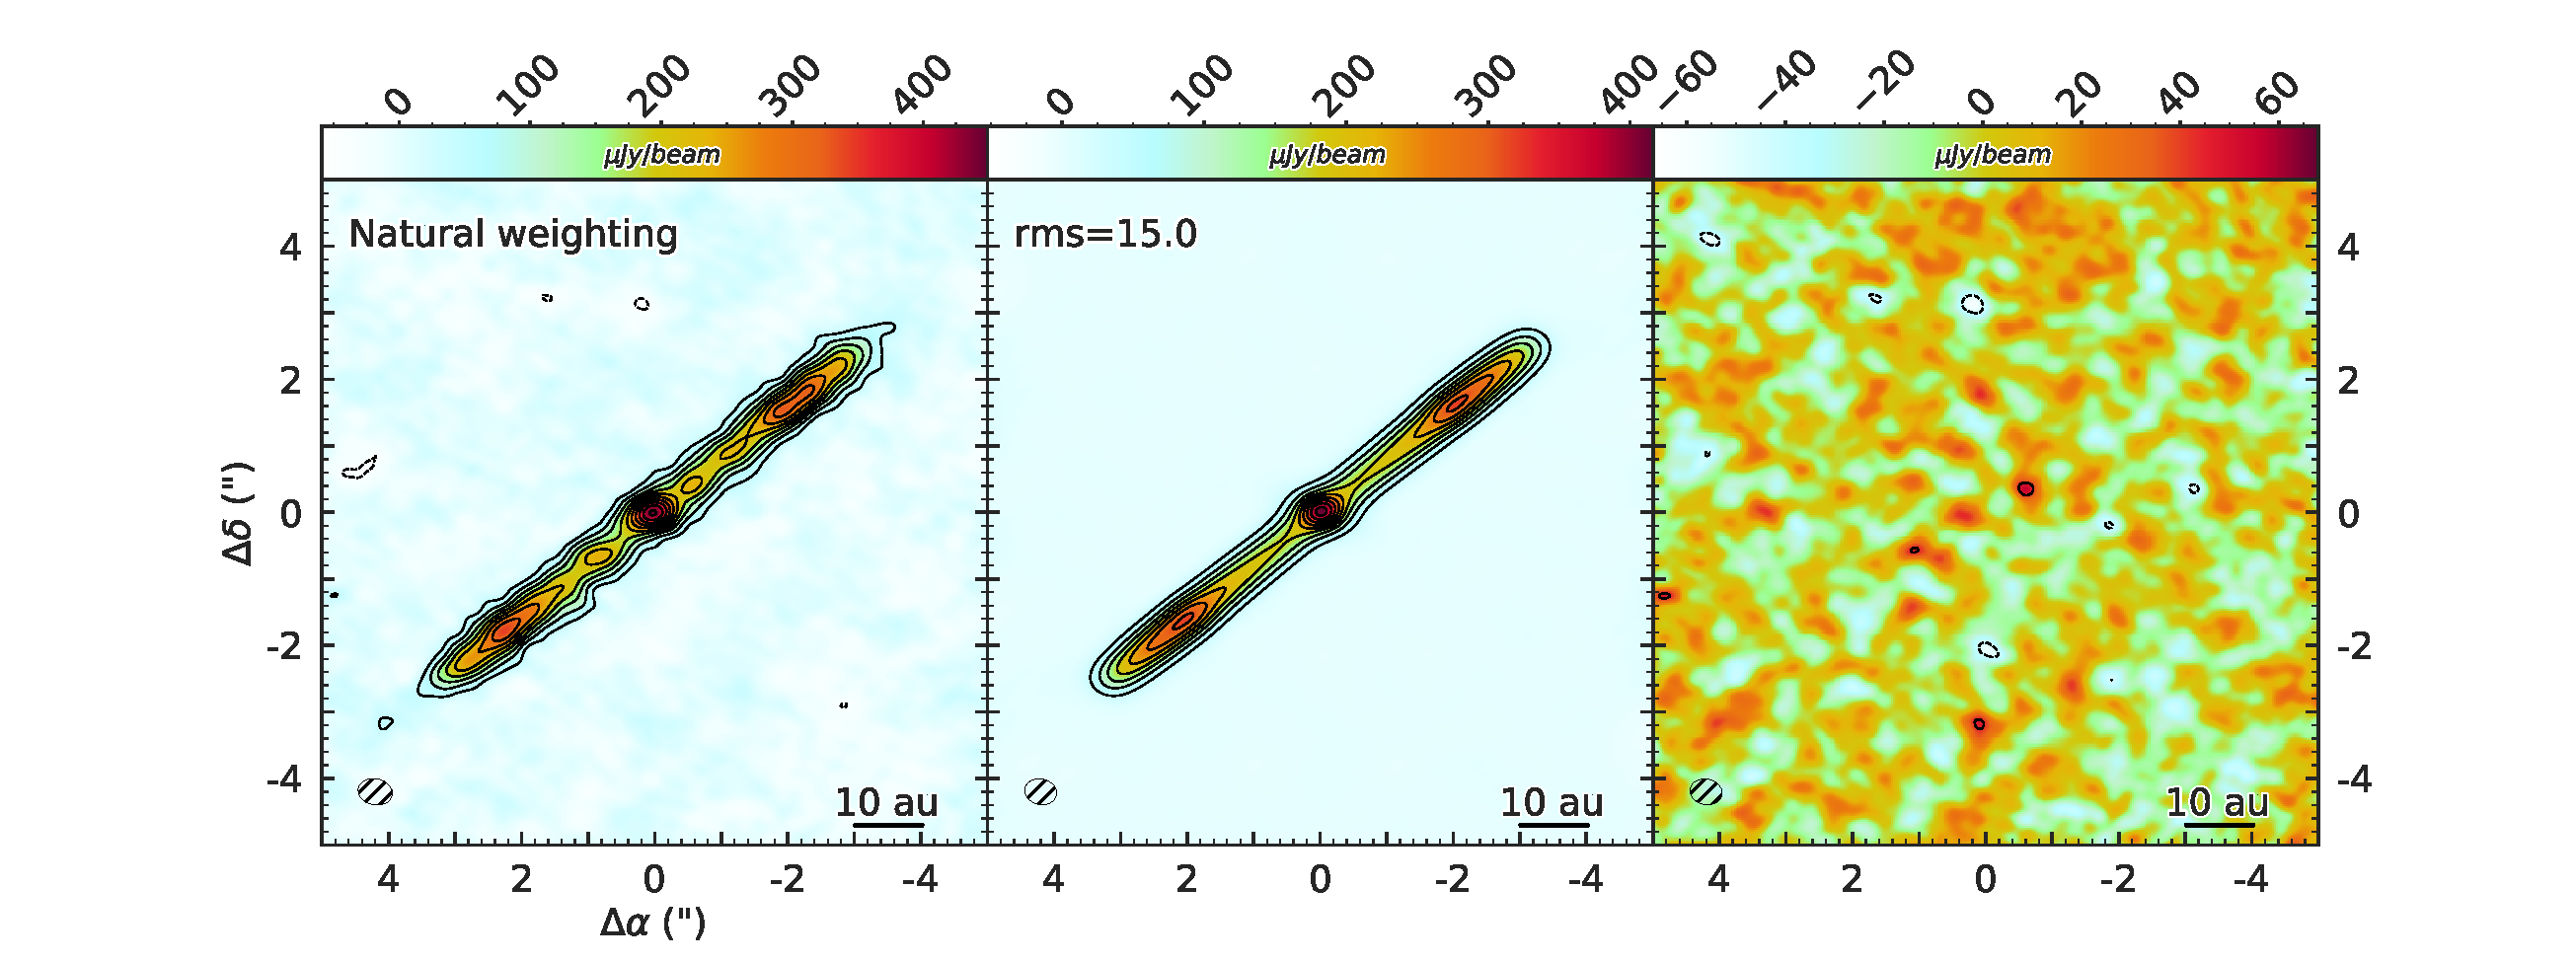
\includegraphics[width=\linewidth]{run6_bestfit_global_concise}
  \caption{(left to right) ALMA observations of AU Mic, best fit model, and best fit model residuals}
  \label{fig:bf}
\end{figure}

This summer we've been investigating the vertical and radial structure of AU Mic using MCMC methods. 
Most parameters are well behaved, but a few questions remain:
  
The posterior for inner radius exhibits severe bimodality, with one solution at $\sim 8$ au and another at $\sim 20$ au. 
A larger inner radius is slightly preferred.
We will be implementing a gap to see how it affects this bimodality.
  
We are still investigating the spatial scales on which our data our sensitive. 
Models with both linear and constant scale height prescriptions prefer values for scale height that do not seem to be lower limits (see Figure \ref{fig:kde}).
% When a model with a linearly increasing scale height is used to fit the data, a very low scale factor ($\sim 0.025$) is preferred; this value does not seem to be a lower limit, as indicated by the posterior distribution in Figure \ref{fig:kde}. 
% Similarly, when a constant scale height model is used to fit the data a scale height of $\sim 1$ au is preferred over smaller values.
We are hoping to further probe the resolution limits of the data by fixing the scale factor at a low value $(\sim 0.003)$ to see if such a constraint requires a worse fit.

\begin{figure}[h]
  \centering
  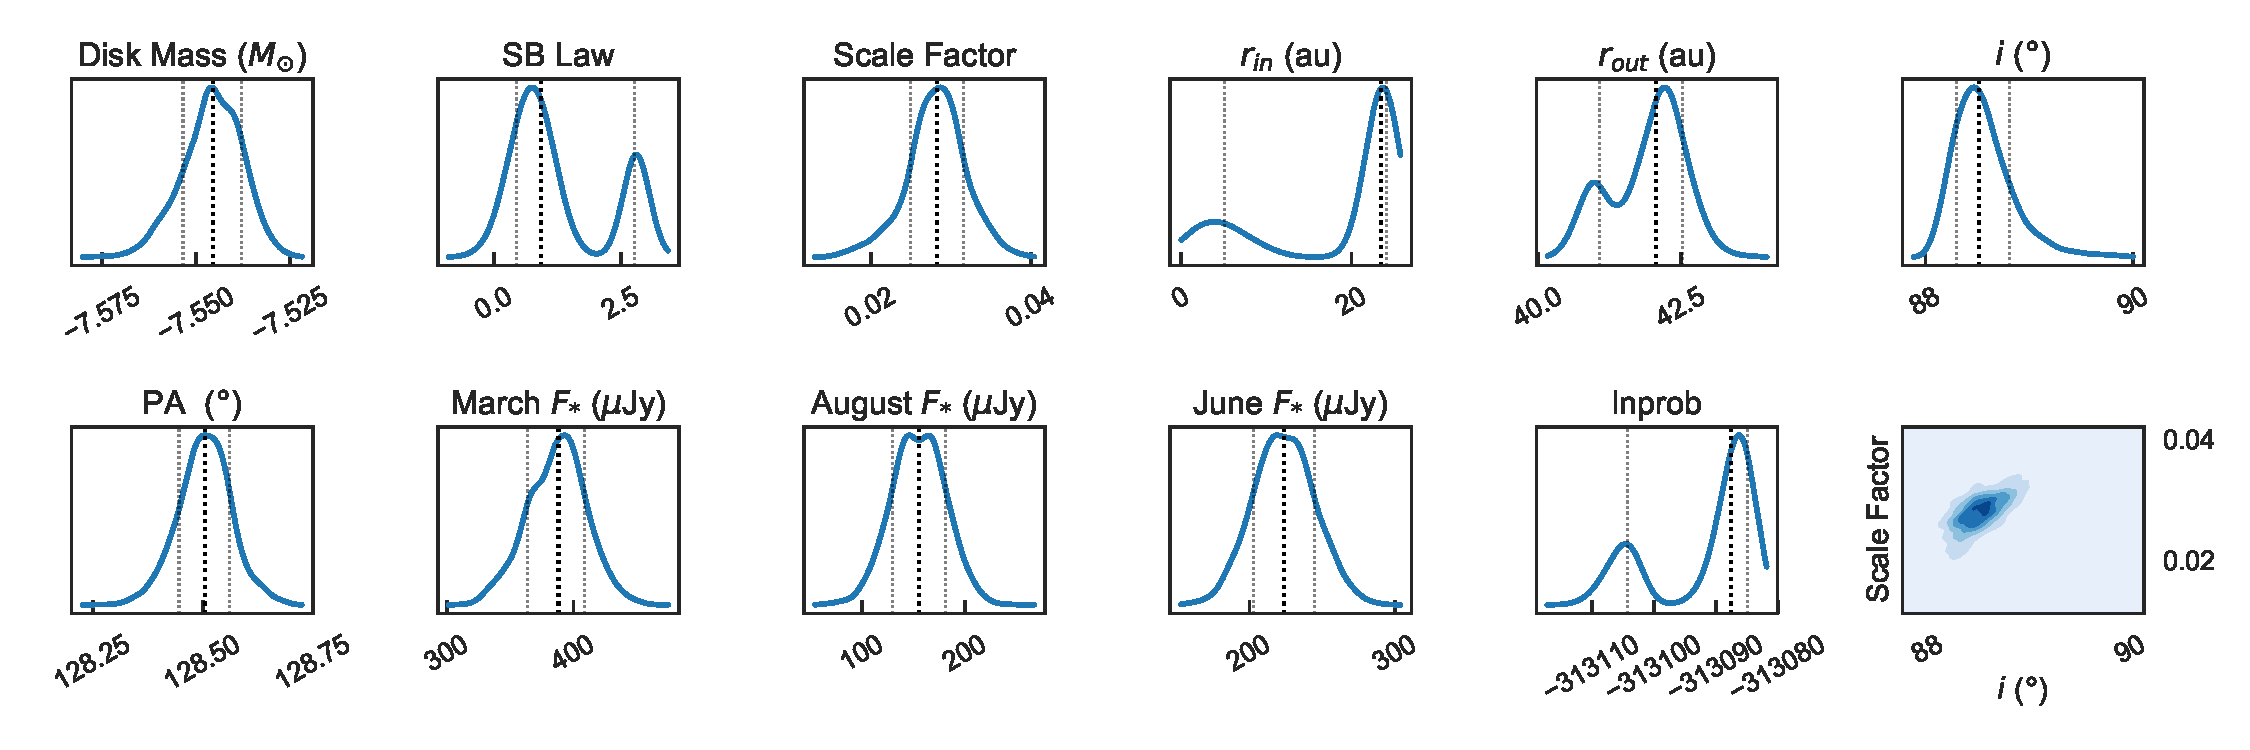
\includegraphics[width=\linewidth]{run6_kde}
  \caption{Posterior distribution of free parameters.}
  \label{fig:kde}
\end{figure}



\end{document}
